
\chapter{Formulación en Química Orgánica}

\section{Introducción}
La Química Orgánica constituye una de las principales ramas de la Química, debido al gran número de compuestos que estudia, los cuales tienen como elemento básico de su constitución molecular el átomo de carbono: de aquí que se la llama con frecuencia Química del Carbono.\\

El número de compuestos en los que entra a formar parte el átomo de carbono es casi innumerable, y cada año se descubren varios miles más. Pensemos en la gran cantidad que existe de proteínas, hormonas, vitaminas, plásticos, antibióticos, perfumes, detergentes, etc., y nos daremos cuenta de que el átomo de carbono es un átomo singular: que puede formar cadenas y combinarse fácilmente con un número reducido de átomos, como son el hidrógeno, el oxígeno, el nitrógeno, los halógenos y unos pocos más.-\\

Algunos de los productos orgánicos que hoy manejamos se conocían en la antigüedad; los fenicios y egipcios extraían colorantes de plantas y moluscos (púrpura) y ciertas sustancias medicinales. También conocían la conversión de la grasa animal en jabón y obtenían alcohol por fermentación de azúcares.\\ 

Hasta que en 1828, el químico alemán \emph{Friedrich Wohler}, logró sintetizar la urea a partir de materiales inorgánicos, se creía que los compuestos orgánicos solo podían producirse por la acción de una "fuerza vital" que únicamente poseían los seres vivos. A partir de entonces se han sintetizado cientos de miles de compuestos orgánicos. Kekulé, Le Bel, Van't Hoff y otros, entre 1850 y 1872, han desarrollado el concepto de enlace químico logrando representar las estructuras tridimensionales de las moléculas. En la actualidad se conocen varios millones de compuestos orgánicos diferentes y el ritmo de crecimiento es de más de cincuenta mil nuevos compuestos por año.

\section{Estudio del Átomo de Carbono} 
La configuración electrónica del átomo de carbono es $1s^22s^22p^2$. Tiene por tanto 4 electrones en su capa de valencia, por lo que según la regla del octete tiende a querer rodearse de 4 electrones mas para adquirir configuración de gas noble. La consecuencia de esta configuración es que el átomo de carbono tiende a formar 4 enlaces covalentes muy estables. En la naturaleza se comprueba que se pueden formar largas repeticiones de átomos de carbono unidos entre si por enlaces covalentes dando lugar a grandes cadenas, que suelen estar completadas mayoritariamente por átomos de Hidrógeno y, en menor medida, por otros átomos tales como oxígeno, nitrógeno, azufre, halógenos o metales. También tiene la característica de poder unirse de tres maneras distintas con otro átomo de carbono:\\

\begin{itemize}
	\item\textbf{Enlace Simple} Se comparten tan solo un par de electrones.
	\item\textbf{Enlace Doble} Se comparten dos pares de electrones.
	\item\textbf{Enlace Triple} Se comparten tres pares de electrones.
\end{itemize}
\section{Representación de los Compuestos Orgánicos}
Debido a la especial característica que tienen los compuestos orgánicos a la hora de formar largas cadenas, se hace indispensable el conocer ya no solo la proporción de elementos dentro del compuesto (C, H, O, N...etc) sino también la estructura que presenta. Para ello existen varias maneras de representar los compuestos organicos:\\
\begin{itemize}
	\item \textbf{Fórmula Empírica} Representa la proporción relativa de los elementos presentes dentro de un compuesto orgánico. 
	\begin{center}
		$(C_2H_3O)_x$
	\end{center}
	\item \textbf{Fórmula Molecular} Representa el número exacto de átomos presentes dentro de un compuesto orgánico. No nos da información acerca de su estructura espacial.
	\begin{center}
		$C_4H_6O_2$
	\end{center}
		\item \textbf{Fórmula Desarrollada} Se representan básicamente todos los enlaces del esqueleto carbonado:
		\begin{figure}[h!]
			\centering
			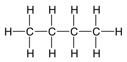
\includegraphics{desarrollada}
		\end{figure}
		\item \textbf{Fórmula Desarrollada} Se representan básicamente los enlaces del esqueleto carbonado y otros importantes, dejando sin desarrollar los de elementos menores (Hidrógenos). Es, con diferencia, la más utilizada en Química Orgánica:
			\begin{figure}[h!]
			\centering
			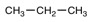
\includegraphics{semides}
		\end{figure}
		Existen también otros tipos de fórmulas que son derivadas de ésta última y que aumentan la esquematicidad de las mismas. Son las llamadas Fórmulas de Línea-Ángulo, donde se representan los enlaces por líneas y los carbonos por ángulos. También es frecuente esquematizar los sustituyentes mediante letras:
		\begin{figure}[h!]
			\centering
			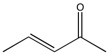
\includegraphics{lineangul}
			\caption{Representación de la \emph{3-penten-2-ona} según la forma línea-ángulo}
		\end{figure}  
\end{itemize}

\section{Número de Carbonos}
La parte más esencial de la nomenclatura orgánica, y que es común a todas las familias de compuestos, es el indicar el número de carbonos presentes en la molécula. Tal es así que, de forma general, se utilizarán una serie de prefijos en griego para denotar el número de carbonos en la molécula:
\begin{table}[h!]
	\centering
	\begin{tabular}{c|c||c|c}
		\textbf{Nº de Carbonos}&\textbf{Prefijos}&\textbf{Nº de Carbonos}&\textbf{Prefijos}\\ \hline
		Met-&1&Hex-&6\\
		Et-&2&Hept-&7\\
		Prop-&3&Oct-&8\\
		But-&4&Non-&9\\
		Pent-&5&Dec-&10\\ \hline
	\end{tabular}
\caption{Prefijos que indican Número de Carbonos}
\end{table}

\section{Hidrocarburos}
Los hidrocarburos son los compuestos orgánicos más sencillos que existen en la naturaleza. Están formados exclusivamente por Carbono e Hidrógeno, pudiendo estar unidos entre si mediante enlaces simples, dobles o triples.
\subsection{Hidrocarburos Saturados: Alcanos o Parafinas}
Son hidrocarburos simples formados por un esqueleto carbonado unido por enlaces simples. También se conocen como Hidrocarburos Saturados. Tienen como fórmula general $C_nH_{2n+2}$. El nombre de los mismos se construye añadiendo a los prefijos que indican el número de Carbonos la terminación \emph{-ano}.

\begin{figure}[h!]
	\centering
	\subfloat[Butano]{
	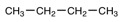
\includegraphics{butano}}
	\hspace{1cm}
	\subfloat[Hexano]{
	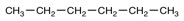
\includegraphics{hexano}}
\end{figure}
Para formular los alcanos (y cualquier compuesto orgánico por extensión) se siguen los siguientes pasos:\\

\begin{itemize}
	\item Se dibuja el esqueleto carbonado dibujando los enlaces C-C con el número de carbonos que indica el nombre de la molécula:
	\begin{center}
		C-C-C-C
	\end{center}
	\item Se completan con hidrógenos los carbonos de forma que llenemos sus cuatro valencias (es decir, nos aseguramos que cada carbono tenga 4 sustituyentes, ya sean hidrógenos, carbonos u otros elementos)
	\begin{figure}[h!]
		\centering
		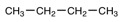
\includegraphics{butano}
	\end{figure}
	
\end{itemize}
\section{Cicloalcanos}
Son Hidrocarburos cuya cadena se encuentra cerrada sobre si misma, formando estructuras geométricas sencillas (triángulos, cuadrados, pentágonos, hexágonos….)
Aunque se pueden utilizar para representarlos la Fórmula Semidesarrollada, es mas usual hacerlo utilizando la Fórmula de Línea-Ángulo. Se nombran de igual manera que los alcanos de cadena abierta pero anteponiendo el prefijo \emph{Ciclo-}.
\begin{figure}[h!]
	\centering
	\subfloat[Ciclopropano]{
		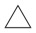
\includegraphics{ciclopropano}}
	\hspace{2cm}
	\subfloat[Ciclopentano]{
		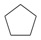
\includegraphics{ciclopentano}}
	\hspace{2cm}
	\subfloat[Ciclohexano]{
	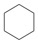
\includegraphics{ciclohexano}}
\end{figure}

\section{Alcanos Ramificados}
Son Alcanos Ramificados aquellos que poseen cadenas secundarias unidas a una cadena que consideramos primaria o principal. La cadena principal se nombra de igual modo que los alcanos y las cadenas secundarias utilizando el prefijo que indica el número de carbonos y la terminación -il. Las ramificaciones solo pueden estar en los carbonos mediales de la molécula, nunca terminales. Hay que recordar que las Fórmulas Orgánicas son representaciones bidimensionales de los compuestos, por lo que las fórmulas orgánicas tal y como las entendemos son una representación estática de un sistema dinámico y complejo, por lo que:

\begin{figure}[h!]
	\centering
	\subfloat[Metilpropano]{
		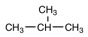
\includegraphics{metilpropano}}
	\hspace{1cm}
	\subfloat[Butano]{
		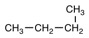
\includegraphics{butano2}}
\end{figure}

Cuando la ramificación pueda estar soportada en mas de un carbono distinto en la cadena principal, se nombra su posición usando números localizadores. Como norma general, entre número y letra se colocará un guión y entre número y número se colocarán comas.

\begin{figure}[h!]
	\centering
	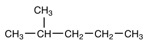
\includegraphics{metilpentano}
	\captionsetup{labelformat=empty}
	\caption{2-metilpentano}
\end{figure}

Los alcanos ramificados presentan tal complejidad a la hora de nombrarlos que es preciso  seguir una serie de normas o reglas establecidas por la IUPAC para la correcta confección de su nombre y su fórmula. Tales reglas son las siguientes:\\

\begin{enumerate}
	
	\item Se toma como cadena principal de la molécula la de mayor número de carbonos. Si hubiese dos cadenas con igual número de carbonos, entonces se tomará como principal la que contenga mayor número de ramificaciones o cadenas secundarias.
	\begin{figure}[h!]
		\centering
		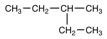
\includegraphics{3metilpentano}
		\captionsetup{labelformat=empty}
		\caption{3-metilpentano (en lugar de 2-etilbutano)}
	\end{figure}
	\item e numera la cadena principal de un extremo a otro de forma que los números localizadores de las cadenas secundarias sean los mas bajos posible
	\begin{figure}[h!]
		\centering
		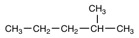
\includegraphics{2metilpentano}
		\captionsetup{labelformat=empty}
		\caption{2-metilpentano (en lugar de 4-metilbutano)}
	\end{figure}
	\item Si hubiese más de una cadena secundaria con el mismo número de átomos de carbono, se antepondrán al nombre los  prefijos de cantidad di-, tri-, tetra-,…
	\begin{figure}[h!]
		\centering
		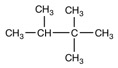
\includegraphics{trimetilbutano}
		\captionsetup{labelformat=empty}
		\caption{2,2,3-trimetilbutano}
	\end{figure}
	\item En caso de que hubiese distintas ramificaciones con distinto número de átomos de carbono, estas se ordenarán siguiendo riguroso orden alfabético. Para ello no se tendrán en cuenta los prefijos multiplicadores si los hubiera.
	\begin{figure}[h!]
		\centering
		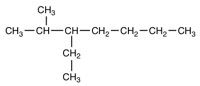
\includegraphics{metiletilheptano}
		\captionsetup{labelformat=empty}
		\caption{2-metil-3-etilheptano}
	\end{figure}
	\item Si en la molécula hubiera una ramificación que tuviera a su vez otra ramificación, estas se nombrarán entre paréntesis sabiendo que se tomará como carbono uno el más próximo a la cadena principal.
	 \begin{figure}[h!]
	 	\centering
	 	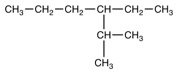
\includegraphics{metiletilhexano}
	 	\captionsetup{labelformat=empty}
	 	\caption{3-(1-metiletil)hexano}
	 \end{figure}
 \setcounter{nx}{\value{enumi}}
\end{enumerate}

\subsection{Hidrocarburos Insaturados (I): Alquenos u Olefinas}

Los Alquenos son hidrocarburos en donde al menos dos de sus carbonos están unidos entre si mediante un enlace doble. Se nombran utilizando los prefijos que indican el número de carbonos en la cadena principal seguido de la terminación \emph{-eno}\\
\begin{figure}[h!]
	\centering
	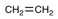
\includegraphics{eteno}
	\captionsetup{labelformat=empty}
	\caption{Eteno (también llamado comúnmente \emph{Etileno})}
\end{figure}

\begin{itemize}

\item Para cadenas mayores de tres átomos de carbono, es imprescindible localizar la posición del doble enlace en la cadena principal:
\begin{figure}[h!]
	\centering
	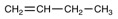
\includegraphics{1buteno}
	\captionsetup{labelformat=empty}
	\caption{1-buteno}
\end{figure}

\item Si en la cadena principal existiese mas de un doble enlace (polieno), estos se nombrarán anteponiendo los prefijos de cantidad a la terminación -eno:

\begin{figure}[h!]
	\centering
	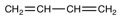
\includegraphics{13butadieno}
	\captionsetup{labelformat=empty}
	\caption{1,3-butadieno}
	\end{figure}
\end{itemize}

\subsection{Hidrocrburos Insaturados (II): Alquinos o Acetilenos}

Los Alquinos son hidrocarburos en donde al menos dos de sus carbonos están unidos entre si mediante un enlace triple. Se nombran utilizando los prefijos que indican el número de carbonos en la cadena principal seguido de la terminación \emph{-ino}.
\begin{itemize}
	
\begin{figure}[h!]
	\centering
	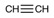
\includegraphics{etino}
	\captionsetup{labelformat=empty}
	\caption{Etino (también llamado comúnmente \emph{Acetileno})}
\end{figure}
	\item Para cadenas mayores de tres átomos de carbono, es imprescindible localizar la posición del triple enlace en la cadena principal:

\begin{figure}[h!]
	\centering
	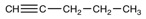
\includegraphics{1pentino}
	\captionsetup{labelformat=empty}
	\caption{1-pentino}
\end{figure}

	\item Si en la cadena principal existiese mas de un triple enlace, estos se nombrarán anteponiendo los prefijos de cantidad a la terminación \emph{-ino}:

\begin{figure}[h!]
	\centering
	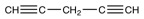
\includegraphics{14pentadiino}
	\captionsetup{labelformat=empty}
	\caption{1,4-pentadiino}
\end{figure}
\end{itemize}
\subsection{Hidrocarburos Insaturados Ramificados}

La introducción tanto de ramificaciones como de insaturaciones en los hidrocarburos hace que el número de compuestos orgánicos formados solamente por Carbono e Hidrógeno crezca de manera exponencial. Es necesario, por tanto, introducir nuevas reglas que se añadan o incluso modifiquen las existentes:\\

\begin{enumerate}
	\setcounter{enumi}{\value{nx}}
	\item La cadena principal será aquella que contenga mayor número de insaturaciones (dobles y triples enlaces). En el caso de que existan dos posibilidades que tengan igual numero de insaturaciones, se cogerá la mas larga. Y a igualdad de átomos de carbono, se escogerá la que contenga más número de dobles enlaces.\\
	
	\item Se numera la cadena principal de un extremo a otro de forma que los números localizadores de las insaturaciones sean lo mas bajos posibles. Si hay coincidencia, se comenzará por el extremo que le asigne números localizadores mas bajos a los dobles enlaces. A la hora de nombrarlos, los triples enlaces se nombran en último lugar.
	\begin{figure}[h!]
		\centering
		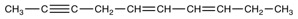
\includegraphics{octendiino}
		\captionsetup{labelformat=empty}
		\caption{3-octen-1,7-diino}
	\end{figure}
	\item Las ramificaciones no tienen prioridad con respecto a las insaturaciones, por lo que se nombran al principio y de acuerdo a las Reglas 3 y 4.
	\begin{figure}[h!]
		\centering
		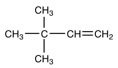
\includegraphics{dimetilbuteno}
		\captionsetup{labelformat=empty}
		\caption{3,3-dimetil-1-buteno}
	\end{figure}
	\item Las insaturaciones que recaigan sobre cadenas secundarias se nombrarán igualmente entre paréntesis y teniendo en cuenta que el carbono uno será el más próximo a la cadena principal.
	\begin{figure}[h!]
		\centering
		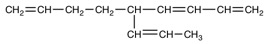
\includegraphics{putada}
		\captionsetup{labelformat=empty}
		\caption{5-(1-propenil)-1,3,8-octatrieno}
	\end{figure}
\end{enumerate}
Cuando tengamos dobles y triples enlaces en la misma molécula, generalmente el prefijo que indica el número de carbonos recae sobre el sufijo del doble enlace:\\

\begin{figure}[h!]
	\centering
	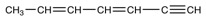
\includegraphics{heptadienino}
	\captionsetup{labelformat=empty}
	\caption{3,5-heptadien-1-ino}
\end{figure}
\subsection{Hidrocarburos Halogenados}
Los Hidrocarburos halogenados, también llamados Haloalcanos o Haluros de Alquilo provienen de sustituir los hidrógenos de un Hidrocarburo (ya sea saturado o insaturado) por halógenos. Dichos halógenos han de ser localizados mediante sus correspondientes números localizadores, siempre que sea necesario.

\begin{figure}[h!]
	\centering
	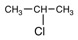
\includegraphics{cloropropano}
	\captionsetup{labelformat=empty}
	\caption{2-Cloropropano}
\end{figure}

